% Slides: Khai thác các mẫu hiếm (Rare Pattern Mining)
% Compile: xelatex main.tex
\documentclass[aspectratio=169,11pt]{beamer}

% ----- Fonts (Vietnamese, xelatex) -----
\usepackage{fontspec}
\usefonttheme{professionalfonts}
\setsansfont{Helvetica Neue}
\setmonofont{Menlo}

% ----- Venue colors: NeurIPS -----
\usepackage{xcolor}
\definecolor{primary}{HTML}{8B5CF6}
\definecolor{accent}{HTML}{2563EB}
\definecolor{darktext}{HTML}{1E1E1E}
\definecolor{okgreen}{HTML}{059669}
\definecolor{warnred}{HTML}{DC2626}

% ----- Theme -----
\usetheme{default}
\usecolortheme{default}
\setbeamercolor{normal text}{fg=darktext}
\setbeamercolor{frametitle}{fg=primary}
\setbeamercolor{title}{fg=primary}
\setbeamercolor{subtitle}{fg=accent}
\setbeamercolor{structure}{fg=accent}
\setbeamercolor{itemize item}{fg=primary}
\setbeamercolor{itemize subitem}{fg=accent}
\setbeamercolor{alerted text}{fg=warnred}
\setbeamerfont{frametitle}{series=\bfseries,size=\Large}
\setbeamerfont{title}{series=\bfseries,size=\LARGE}
\setbeamertemplate{navigation symbols}{}
\setbeamertemplate{footline}{%
  \hfill{\color{gray}\insertframenumber/\inserttotalframenumber}\hspace{3mm}\vspace{2mm}%
}
\setbeamertemplate{itemize item}{\textbullet}
\setbeamertemplate{itemize subitem}{--}

% ----- Packages -----
\usepackage{graphicx,amsmath,booktabs}
\graphicspath{{figures/}}

% ----- Metadata -----
\title{Khai thác các mẫu hiếm\\ (Rare Pattern Mining)}
\subtitle{Bài tập lớn môn Khai thác dữ liệu nâng cao}
\author{[Họ tên sinh viên --- MSSV]}
\institute{}
\date{Tháng 6 năm 2026}

\begin{document}

% ============ Slide 1: Title ============
\begin{frame}
\titlepage
\note{Chờ giới thiệu. ``Em xin chào thầy/cô và các bạn. Hôm nay em trình bày đề tài
Khai thác các mẫu hiếm --- Rare Pattern Mining.'' (0:15)}
\end{frame}

% ============ Slide 2: Outline ============
\begin{frame}{Nội dung trình bày}
\begin{itemize}\itemsep0.7em
  \item Bài toán \& động cơ
  \item Ba định nghĩa mẫu hiếm
  \item Ba thuật toán: \textbf{AprioriRare}, \textbf{AprioriInverse}, \textbf{CORI}
  \item Độ đo tương quan \& tính null-invariance
  \item Cài đặt, kiểm chứng tự động, thực nghiệm UCI Mushroom
\end{itemize}
\note{Lướt nhanh 5 phần: lý thuyết định nghĩa, thuật toán, độ đo, rồi phần thực hành
tự cài đặt và thực nghiệm. (0:20) Chuyển: ``Bắt đầu từ câu hỏi vì sao cần mẫu hiếm.''}
\end{frame}

% ============ Slide 3: Motivation ============
\begin{frame}{Động cơ: mẫu hiếm nhưng giá trị cao}
\begin{itemize}\itemsep0.7em
  \item Y tế: tổ hợp triệu chứng bệnh hiếm $\Rightarrow$ giá trị chẩn đoán cao
  \item Công nghiệp: lỗi sản phẩm hiếm gặp = đối tượng cần phát hiện
  \item An ninh mạng: bất thường = hiếm theo định nghĩa
  \item[]
  \item \alert{FIM truyền thống bỏ qua hoàn toàn các mẫu này}
\end{itemize}
\note{Mở bằng câu hỏi: ``Điều thú vị nhất trong dữ liệu có phải là điều xảy ra thường
xuyên nhất không?'' FIM ngầm coi phổ biến = đáng quan tâm --- giả định này sai trong
y tế, công nghiệp, an ninh. (1:00) Chuyển: ``Vậy sao không hạ thấp ngưỡng hỗ trợ?''}
\end{frame}

% ============ Slide 4: Problem ============
\begin{frame}{Vấn đề: hạ minsup là không đủ}
\begin{itemize}\itemsep0.7em
  \item Giải pháp ngây thơ: hạ thấp $minsup$
  \item Hệ quả 1: \textbf{bùng nổ tổ hợp} số itemset
  \item Hệ quả 2: nhiễu --- nhiều ``mẫu hiếm'' có $sup = 0$ (không tồn tại!)
  \item[]
  \item Cần: định nghĩa chặt chẽ + thuật toán riêng + độ đo lọc mẫu giả
\end{itemize}
\note{Hạ minsup làm phần trên của dàn itemset bùng nổ; tệ hơn, nhiều itemset không
phổ biến thậm chí không xuất hiện trong dữ liệu. Ba mảnh ghép của lời giải chính là
ba phần tiếp theo. (1:00) Chuyển: ``Để nói chuyện cụ thể, em dùng một ví dụ nhỏ.''}
\end{frame}

% ============ Slide 5: Running example ============
\begin{frame}{Ví dụ}
\centering
\begin{tabular}{cl}
\toprule
\textbf{Giao dịch} & \textbf{Các mục} \\
\midrule
T1 & pasta, lemon, bread, orange \\
T2 & pasta, lemon \\
T3 & pasta, orange, cake \\
T4 & pasta, lemon, orange, cake \\
\bottomrule
\end{tabular}
\vspace{1em}
\begin{itemize}
  \item $minsup = 2$ $\Rightarrow$ \textbf{11} itemset phổ biến
  \item \{bread\}: $sup = 1$ \quad\textbullet\quad \{bread, cake\}: $sup = 0$
  \item Dùng để chạy tay \& kiểm chứng cài đặt
\end{itemize}
\note{CSDL 4 giao dịch theo bài giảng. Pasta có mặt mọi giao dịch --- nhớ chi tiết này,
nó sẽ quay lại ở phần mẫu giả. (0:45) Chuyển: ``Trên ví dụ này, hiếm nghĩa là gì?''}
\end{frame}

% ============ Slide 6: Three definitions ============
\begin{frame}{Ba định nghĩa mẫu hiếm}
\begin{itemize}\itemsep0.6em
  \item \textbf{Infrequent}: $sup(X) < minsup$ --- bùng nổ, chứa cả $sup = 0$
  \pause
  \item \textbf{Minimal rare (mRI)}: hiếm, \textbf{mọi tập con đều phổ biến}\\
        {\color{accent}$\Rightarrow$ biên dưới của vùng hiếm trong dàn itemset}
  \pause
  \item \textbf{Perfectly rare (PRI)}: $minsup \le sup < maxsup$,\\
        mọi item thành phần đều hiếm
  \pause
  \item[]
  \item Ví dụ ($minsup=2$): mRI = \{bread\}, \{lemon, cake\} \quad\textbullet\quad PRI = \{bread\}
\end{itemize}
\note{Tâm điểm lý thuyết. Hình ảnh chính: dàn itemset chia hai vùng bởi một đường
biên; mRI là các điểm hiếm đầu tiên ngay khi vượt biên --- nhỏ gọn mà đại diện được
mọi mẫu hiếm. PRI thêm ngưỡng dưới để loại nhiễu và đòi mọi item cũng hiếm. (1:15)
Chuyển: ``Mỗi định nghĩa có một thuật toán tương ứng.''}
\end{frame}

% ============ Slide 7: AprioriRare ============
\begin{frame}{AprioriRare: tìm biên hiếm tối thiểu}
\begin{itemize}\itemsep0.6em
  \item Duyệt theo mức (level-wise) như Apriori
  \item Ứng viên sống sót qua prune mà không phổ biến \textbf{$\Rightarrow$ chính là mRI}
  \item Itemset hiếm không dùng sinh ứng viên tiếp
  \item[]
  \item Ví dụ: mRI = \textbf{\{bread\}, \{lemon, cake\}} \quad {\color{okgreen}khớp bài giảng}
  \item \alert{Nhược: phải duyệt toàn bộ vùng phổ biến}
\end{itemize}
\note{Điểm tinh tế: ứng viên đã qua prune nghĩa là mọi tập con $k-1$ đều phổ biến,
và theo anti-monotone mọi tập con nhỏ hơn cũng vậy --- nên hễ không phổ biến là tự
động thành mRI, không cần kiểm tra thêm. Nhược điểm chi phí sẽ được định lượng ở
thực nghiệm A. (1:15) Chuyển: ``Thuật toán thứ hai đi theo hướng ngược lại.''}
\end{frame}

% ============ Slide 8: AprioriInverse ============
\begin{frame}{AprioriInverse: thu hẹp ngay từ đầu}
\begin{itemize}\itemsep0.6em
  \item Hai ngưỡng $(minsup, maxsup)$
  \item \textbf{Loại mọi item phổ biến ngay bước khởi tạo}
  \item Đúng đắn: mọi item hiếm $\Rightarrow$ mọi tập con hiếm (điều kiện PRI tự thoả)
  \item \alert{Đổi lại: bỏ sót mẫu lai \{item hiếm + item phổ biến\}}
  \item[]
  \item Ví dụ $(1.1,\ 3.1)$: 5 PRI \quad {\color{okgreen}khớp bài giảng}
\end{itemize}
\note{Đối lập với AprioriRare: vứt bỏ item phổ biến từ đầu nên không gian tìm kiếm
nhỏ hơn hẳn. Cái giá: mẫu lai như \{bệnh hiếm, triệu chứng phổ biến\} nằm ngoài tầm
với. (1:00) Chuyển: ``Hiếm thôi chưa đủ --- mẫu tìm được có đáng tin không?''}
\end{frame}

% ============ Slide 9: Spurious patterns ============
\begin{frame}{Mẫu giả: phổ biến $\ne$ đáng tin}
\begin{itemize}\itemsep0.7em
  \item \{pasta, cake\} xuất hiện ở \textbf{50\%} giao dịch
  \item Nhưng pasta có mặt trong \textbf{mọi} giao dịch
  \item Đồng xuất hiện là tất yếu --- \alert{không có liên hệ thật} (spurious)
  \item[]
  \item Cần độ đo tương quan để lọc
\end{itemize}
\note{Chuyển mạch sang nửa sau của câu chuyện. Pasta xuất hiện khắp nơi nên đi cùng
bất cứ thứ gì --- support cao không nói lên mối liên hệ nào. (0:45)
Chuyển: ``Bài giảng giới thiệu hai độ đo chính.''}
\end{frame}

% ============ Slide 10: bond & all-confidence ============
\begin{frame}{Hai độ đo: bond và all-confidence}
\begin{itemize}\itemsep0.55em
  \item $bond(X) = \dfrac{sup(X)}{dsup(X)}$ --- tỉ lệ giao dịch ``liên quan'' chứa toàn bộ $X$
  \item $bond = 1$: các mục \textbf{luôn} đi cùng nhau
  \item $allconf(X) = \dfrac{sup(X)}{\max_{i \in X} sup(\{i\})}$ --- confidence \textbf{nhỏ nhất} của mọi luật từ $X$
  \item Cả hai: $=1$ với itemset đơn; \textbf{anti-monotone} $\Rightarrow$ cắt tỉa kiểu Apriori
  \item[]
  \item Ví dụ: $bond(\{cake, bread\}) = 0$ \quad\textbullet\quad $bond(\{pasta, orange\}) = 3/4$
\end{itemize}
\note{dsup là support tuyển: số giao dịch chứa ít nhất một mục. Nhấn tính
anti-monotone --- CORI sẽ dùng nó để cắt tỉa cả nhánh. All-confidence còn rẻ:
chỉ cần support item đơn tính sẵn một lần. (1:00)
Chuyển: ``Vì sao không dùng lift hay chi bình phương quen thuộc?''}
\end{frame}

% ============ Slide 11: Null-invariance ============
\begin{frame}{Null-invariance: vì sao lift thất bại}
\begin{itemize}\itemsep0.7em
  \item Null transaction: giao dịch không chứa mục nào của mẫu
  \item $\chi^2$, lift bị \alert{bóp méo} bởi hàng triệu giao dịch không liên quan
  \item bond, all-confidence, cosine, Kulczynski: \textbf{null-invariant}
  \item[]
  \item Mẫu hiếm $\subset$ phần rất nhỏ dữ liệu $\Rightarrow$ \textbf{bắt buộc} dùng null-invariant
\end{itemize}
\note{Lý do sâu xa để chọn bond/all-confidence cho mẫu hiếm: mẫu hiếm theo định nghĩa
chỉ chạm một phần rất nhỏ dữ liệu, phần còn lại toàn null transactions --- độ đo nào
nhạy với chúng sẽ bị thổi phồng hoặc bóp méo trên dữ liệu thưa. (0:45)
Chuyển: ``Hai dòng kỹ thuật --- hiếm và tương quan --- hội tụ ở CORI.''}
\end{frame}

% ============ Slide 12: CORI ============
\begin{frame}{CORI: hiếm + tương quan trong một lần duyệt}
\begin{itemize}\itemsep0.55em
  \item Rare correlated: $sup(X) < maxsup$ \textbf{và} $bond(X) \ge minbond$
  \item Hai ràng buộc đối ngẫu: hiếm = \textbf{monotone} \quad\textbullet\quad bond = \textbf{anti-monotone}
  \item Duyệt kiểu Eclat, mỗi itemset giữ \textbf{TID-List + DTID-List}
  \item bond rớt ngưỡng $\Rightarrow$ cắt cả nhánh; $sup \ge maxsup$ $\Rightarrow$ chưa xuất nhưng vẫn mở rộng
  \item[]
  \item Ví dụ $(3,\ 0.6)$: \textbf{\{bread\}, \{cake\}, \{orange, cake\}} \quad {\color{okgreen}khớp bài giảng}
\end{itemize}
\note{Đỉnh lý thuyết của bài. Khi nối hai itemset: TID-List lấy giao, DTID-List lấy
hợp --- support và bond của itemset mới tính ngay không cần quét lại CSDL. Lưu ý
thiết kế: nút chưa hiếm vẫn phải mở rộng vì tập cha có thể hiếm --- khác cắt tỉa
support truyền thống. (1:15) Chuyển: ``Toàn bộ lý thuyết trên được em cài đặt lại
và kiểm chứng tự động.''}
\end{frame}

% ============ Slide 13: Implementation & verification ============
\begin{frame}{Cài đặt \& kiểm chứng 100\%}
\begin{itemize}\itemsep0.6em
  \item Python 3.13, \textbf{chỉ thư viện chuẩn}; TID-set dùng chung cho cả 3 thuật toán
  \item \textbf{19 assert} đối chiếu từng con số kỳ vọng trên ví dụ --- {\color{okgreen}\textbf{100\% ĐẠT}}
  \item Phủ FIM, AprioriRare, AprioriInverse, CORI \& các độ đo
  \item[]
  \item \{pasta, cake\}: $lift = 1.0$, $bond = 0.5$ $\Rightarrow$ xác nhận mẫu giả bằng số
\end{itemize}
\note{19 assert phủ toàn bộ: bảng FIM, ba thuật toán, bond, all-confidence,
TID/DTID-List --- tất cả khớp kết quả tính tay trên ví dụ minh họa. Bảng độ đo cặp
xác nhận bằng số trực giác mẫu giả ở slide 9. (1:00)
Chuyển: ``Trên dữ liệu thật thì các đánh đổi lý thuyết hiện ra thế nào?''}
\end{frame}

% ============ Slide 14: Exp A (figure) ============
\begin{frame}{Exp A --- Cái giá của việc đi xuyên vùng phổ biến}
\centering

\includegraphics[width=\textwidth,height=0.62\textheight,keepaspectratio]{mushroom_runtime.png}
\vspace{0.4em}
\begin{itemize}
  \item UCI Mushroom: 8\,124 giao dịch, 118 item (dữ liệu dày)
  \item $minsup$ 0.6 $\to$ 0.2: \#frequent tăng \textbf{$\sim$890$\times$} (51 $\to$ 45\,391); \#mRI chỉ \textbf{$\sim$8$\times$} (122 $\to$ 986)
\end{itemize}
\note{Đọc biểu đồ: thời gian AprioriRare tăng theo cấp mũ khi minsup giảm. mRI là
biểu diễn biên gọn --- nhưng chi phí tính nó bị chi phối bởi kích thước vùng phổ
biến, đúng như dự báo ở slide 7. Đây là lý do các nghiên cứu mới dùng metaheuristic
hoặc bit dọc để né duyệt vét cạn. (1:00)}
\end{frame}

% ============ Slide 15: Exp B & C (figure) ============
\begin{frame}{Exp B \& C --- PRI rẻ, CORI giàu ngữ nghĩa}
\centering
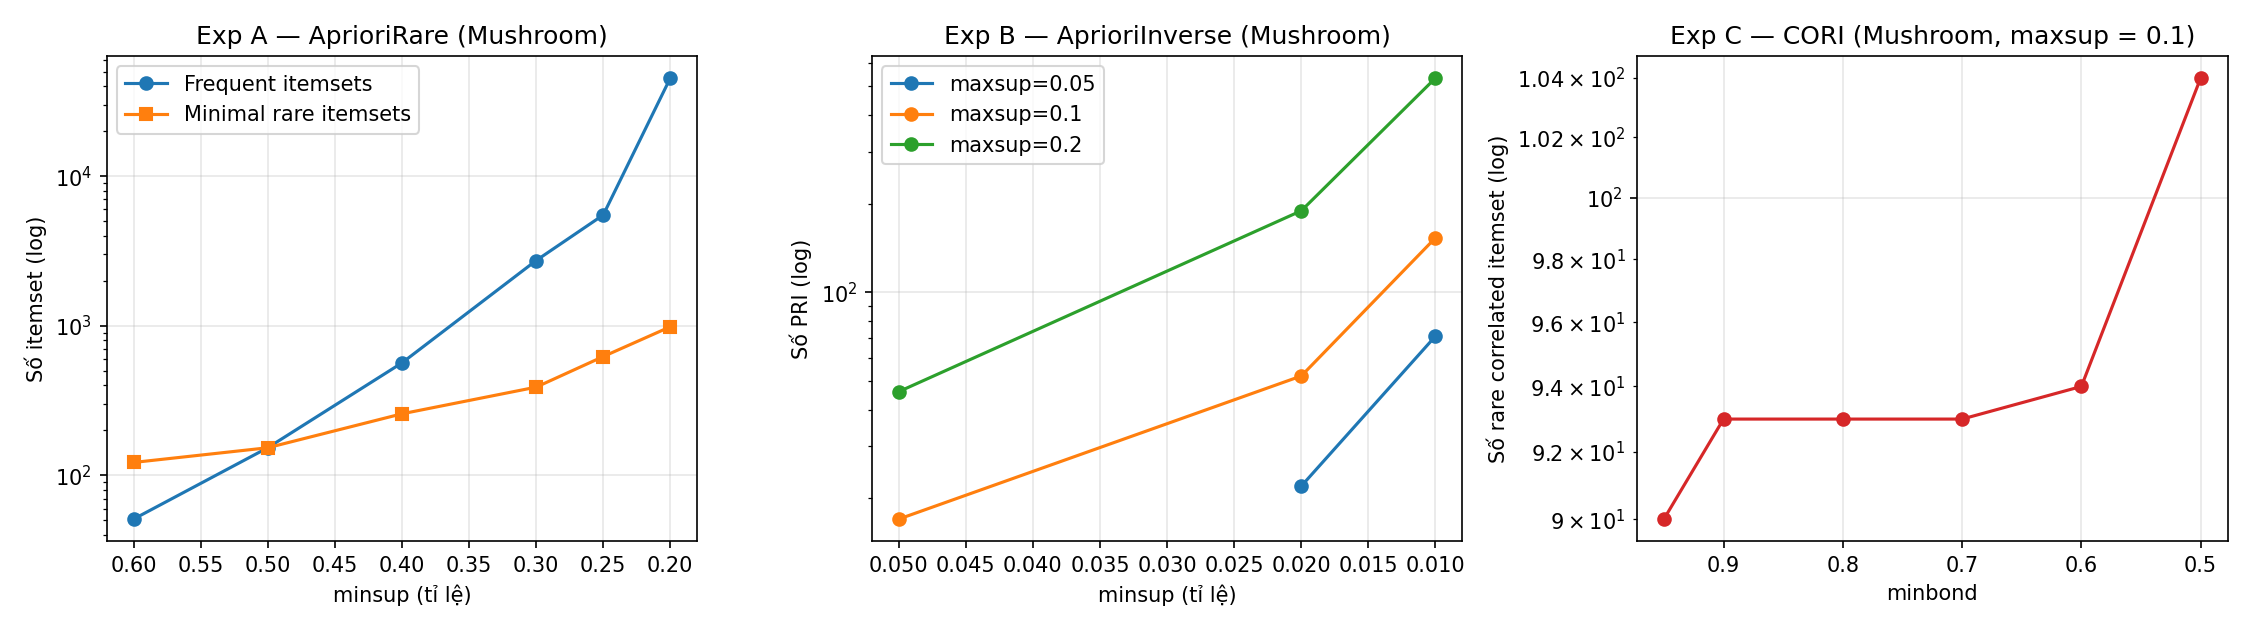
\includegraphics[width=\textwidth,height=0.60\textheight,keepaspectratio]{mushroom_experiments.png}
\vspace{0.3em}
\begin{itemize}
  \item AprioriInverse: \textbf{mili-giây} --- alphabet hiếm rất nhỏ (bài toán khác, không phải benchmark cùng điều kiện)
  \item CORI: bão hòa 90--104 mẫu khi nới $minbond$ 0.95 $\to$ 0.5; mẫu \textbf{$bond = 1.0$}: \{odor=m, \dots\}, $sup = 36$ (0.44\%)
\end{itemize}
\note{AprioriInverse nhanh hơn 2--3 bậc vì bước loại item phổ biến vứt bỏ phần lớn
alphabet --- nhưng nhấn mạnh: hai bài toán khác nhau, không so sánh trực tiếp.
Mẫu đắt giá nhất của CORI: 36 cây nấm mùi mốc luôn đồng thời không vòng cuống và
cuống màu quế --- bond bằng 1 tuyệt đối, loại tri thức FIM không bao giờ chạm tới.
(1:15) Chuyển: ``Ba thực nghiệm chốt lại ba đánh đổi.''}
\end{frame}

% ============ Slide 16: Conclusion ============
\begin{frame}{Kết luận: ba đánh đổi}
\begin{itemize}\itemsep0.7em
  \item \textbf{mRI gọn nhưng đắt} --- phải duyệt toàn vùng phổ biến
  \item \textbf{PRI rẻ nhưng hẹp} --- bỏ sót mẫu lai
  \item \textbf{CORI cân bằng} --- ràng buộc kép, kết quả nhỏ \& giàu ngữ nghĩa
  \item[]
  \item Hướng 2021--2026: metaheuristic (MRI-CE), fuzzy, utility, \textbf{privacy}
\end{itemize}
\note{Thông điệp mang về: không có định nghĩa hiếm ``đúng'' duy nhất --- chỉ có đánh
đổi giữa độ phủ và chi phí; và trên dữ liệu thưa, null-invariance là bắt buộc.
Hướng phát triển nổi bật nhất là privacy: chính vì hiếm, mẫu hiếm dễ định danh cá
nhân hơn. (0:50)}
\end{frame}

% ============ Slide 17: Thank you ============
\begin{frame}{Cảm ơn \& Hỏi đáp}
\centering
\vspace{1em}
{\Large\color{primary}\textbf{Xin cảm ơn thầy/cô và các bạn!}}\\[1.5em]
{\large 3 định nghĩa \quad\textbullet\quad 3 thuật toán \quad\textbullet\quad kiểm chứng 100\% \quad\textbullet\quad UCI Mushroom}\\[2em]
Mã nguồn \& kết quả: \texttt{advantage\_data\_mining/code}, \texttt{results/}\\[2em]
{\Large Mời thầy/cô và các bạn đặt câu hỏi}
\note{Cảm ơn, mời câu hỏi. (0:20) Chuẩn bị sẵn các câu trả lời trong TALK\_SCRIPT.md:
so sánh AprioriRare/Inverse, vì sao giới hạn kích thước 4 ở CORI, vì sao không dùng
lift, khả năng mở rộng sang dữ liệu Việt Nam.}
\end{frame}

\end{document}
